The main goal of the jumper is (without much of a surprise) to jump as high as possible.
This example was designed to introduce the \emph{bioptim}'s ability to reduce the number of degrees-of-freedom (DoF) of a model via the mappings, to include nonlinear boundaries on the controls, and to solve complex multiphase programs that include impacts and free time phases.

The model used is a full body model consisting of 3 DoF at the pelvis (the forward and upward translation, and the tranverse rotation), 2 DoF at each upper limb (shoulder flexion and abduction), and 3 DoF at each lower limb (hip, knee and ankle flexion) for a total of 13 DoF.
For this optimization, the \emph{BidirectionalMapping} is used to ignore the shoulder abduction---by setting the mapping to \emph{None}---and to symmetrize the left-hand and right-hand sides, effectively creating a 7 DoF pseudo-2D model. 
Since this is a full body model, the root segment (i.e., the pelvis) is left uncontrolled, reducing the number of control variables to 4, namely the shoulder, hip, knee and ankle flexions. 

A total of five phases are used to describe the dynamics of the jump and landing. 
The first two consists in a phase with two (i.e., heel and toe) and one (i.e., toe) contacts on the ground, respectively. 
A contact is described as a point where forces can be applied to nullify the accelerations. 
The aerial phase is free-fall dynamics, that is a dynamics without contact points.
The last two phases (i.e., the reception phase) are the opposite of the push off phase, i.e., a phase with one contact point to the ground (i.e., toe) and then a phase with two contact points (i.e., heel and toe).
The transitions between the phases with less contact points toward more contact points are approximated by the build-in inelastic impact \emph{PhaseTransition}, which recomputes the segment velocities post impact.

The main objective function is a Mayer objective computed at the end of the pushoff phase consisting in maximizing the jumps height ($h$) such that:
\[
h = \frac{\dot{CoM_z^2}}{-2 g} + CoM_z
\]
where $CoM_z$ and $\dot{CoM_z}$ are the center of mass position and velocity, respectively, and $g$ is the gravitional acceleration constant ($\SI{-9.81}{\meter/\second^2}$).
Since `bioptim` minimizes objective, instead of maximizing them, a negative weight is applied to the function. 
Two additional objective are added to facilitate the convergence of the solver.
The first is a minimization of the derivative of the velocities, preventing from large movements during the aerial and reception phases. 
The second is to minimize the each phase time.
Both of these objective have a small weight---four order of magnitude smaller than jump height---so they are not prioritized.
Finally, the end (i.e., the last node of the last phase) pose and velocities of the model are a Mayer objective function so that the model is more or less static, standing knee flexed with its arm horizontally raised. 

\comment{
$\mathcal{J} = XXX$.
% \addtag
% \label{eq:cost_jumper}
}{Add the equations?}

Several constraints are necessary to describe a realistic jump.
The generalized coordinates---i.e., the maximum flexibility expected---are bounded to human-like limits.
The generalized velocities are arbitrarily bounded to $[-10 \pi; 10 pi]$.
The genelized forces are bounded by the torque/position/velocity relashionship measured on a high level athlete using an isokinetic dynamometer (Fig.~\ref{fig:graph_force_vitesse_longueur}). 
For the contact forces from the contact points, a directional constraint is applied such that the force is alway pointing upward, meaning that the model is not allowed to pull on the floor. 
The lateral force norm is constrained to be below the half of the upward force, i.e., the model remain in a cone of friction more or less corresponding in a normal surface contacting shoes. 
\comment{The time of the phases were constraints as such}{C'est pertinent?}
Finally, some constraint were added to prevent the gradient descending solve from exploring non interesting ideas. 
A first one is that during the push off and reception phases, the heel must remain over the floor.
A second is that the center of mass velocity must point upward when leaving the floor, and finally, at the same instant, the arms must be frontward. 

\begin{figure}[h!]
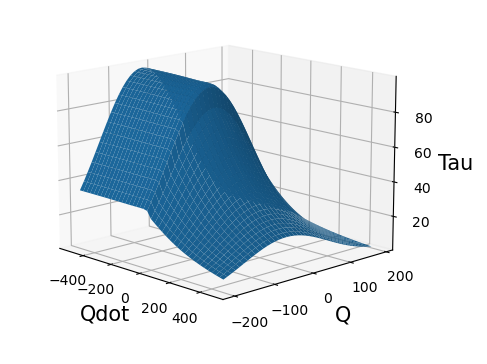
\includegraphics[width=\columnwidth]{figures/graph_force_vitesse_longueur.png}\\
\caption{Surface representing the nonlinear constraint for torque/position/velocity relationship}
\label{fig:graph_force_vitesse_longueur}
\end{figure}

To accelerate solving the problem using \emph{ipopt}, the problem was first approximately solved using the BFGS hessian approximation for 200 iterations maximum.
Then, the solution was re-optimized, from that solution, with an exact-hessian computations for up to 1000 iterations.

The optimized solution of a \SI{1.35}{\meter} jump height was obtained in \SI{0}{\second}.
The solution reproduced a human proximo-distal strategy, that is activating large segments first (for instance the torso) and adding sequentially the more distal segments, the most distal---and the consequently the last to activate---being the ankle.

